%
% VorlagePraxisbericht.tex		
% 	
% Florian Kalinke
% 09.09.2013
%				
% Daniel Betsche	
% 05.09.2014 					

\documentclass[pdftex,12pt,a4paper]{article}

\usepackage[utf8]{inputenc}
\usepackage[ngerman]{babel}
\usepackage[T1]{fontenc}
\usepackage[pdftex]{graphicx}
\usepackage{float}
\usepackage{tabularx}
\usepackage{multirow}
\usepackage[hyphens]{url}
\usepackage{geometry}
\geometry{a4paper,left=25mm,right=25mm, top=1cm, bottom=25mm, includeheadfoot}
\usepackage{fancyhdr}
\usepackage{setspace}
\usepackage[usenames, dvipsnames]{color}
\usepackage{listings}	% for code
\usepackage{xcolor}
%\usepackage{hyperref}  % auskommentieren um verlinkungen zu ermöglichen
\lstset{language=Java}

\onehalfspacing	% Zeilenabstand erhöhen

% Kopf- und Fußzeilen einbinden
\pagestyle{fancy}
\fancyhf{}
\fancyhead[R]{Seite \thepage}
\renewcommand{\headrulewidth}{0.5pt}

% Schriftart auf Arial setzen
\renewcommand{\rmdefault}{phv} % Arial
\renewcommand{\sfdefault}{phv} % Arial

\begin{document}
% Um Java Code einzubinden
\definecolor{javared}{rgb}{0.6,0,0} % for strings
\definecolor{javagreen}{rgb}{0.25,0.5,0.35} % comments
\definecolor{javapurple}{rgb}{0.5,0,0.35} % keywords
\definecolor{javadocblue}{rgb}{0.25,0.35,0.75} % javadoc

% Um XML Code einzubinden
\definecolor{gray}{rgb}{0.4,0.4,0.4}
\definecolor{darkblue}{rgb}{0.0,0.0,0.6}
\definecolor{cyan}{rgb}{0.0,0.6,0.6}

% Die lstlisting style Definitionen
\colorlet{punct}{red!60!black}
\definecolor{background}{HTML}{EEEEEE}
\definecolor{delim}{RGB}{20,105,176}
\colorlet{numb}{magenta!60!black}

% http://tex.stackexchange.com/questions/10255/xml-syntax-highlighting
\lstset{
	basicstyle=\ttfamily,
	columns=fullflexible,
	showstringspaces=false,
	commentstyle=\color{gray}\upshape
}
\lstdefinelanguage{XML}
{
	basicstyle=\normalfont\ttfamily\bfseries,
	morestring=[b]",
	morestring=[s]{>}{<},
	morecomment=[s]{<?}{?>},
	stringstyle=\color{black},
	identifierstyle=\color{delim},
	keywordstyle=\color{delim},
	breaklines=true,
  frame=lines,
  backgroundcolor=\color{background},
	morekeywords={
		xmlns,version,type,properties,key,name,description,type,values,property
	}% list your attributes here
}
% http://texblog.org/2011/06/11/latex-syntax-highlighting-examples/
\lstdefinestyle{customjava}{
	language=Java,
	basicstyle=\normalfont\ttfamily,
	keywordstyle=\color{javapurple}\bfseries,
	stringstyle=\color{javared},
	commentstyle=\color{javagreen},
	morecomment=[s][\color{javadocblue}]{/**}{*/},
	numbers=none,
	stepnumber=2,
	numbersep=10pt,
	frame=lines,
	backgroundcolor=\color{background},
	tabsize=4,
	showspaces=false,
	showstringspaces=false
}
% http://tex.stackexchange.com/questions/83085/how-to-improve-listings-display-of-json-files
\lstdefinelanguage{json}{
    basicstyle=\normalfont\ttfamily,
    numbers=none,
    numberstyle=\scriptsize,
    stepnumber=1,
    numbersep=10pt,
    showstringspaces=false,
    breaklines=true,
    frame=lines,
    backgroundcolor=\color{background},
    literate=
     *{0}{{{\color{numb}0}}}{1}
      {1}{{{\color{numb}1}}}{1}
      {2}{{{\color{numb}2}}}{1}
      {3}{{{\color{numb}3}}}{1}
      {4}{{{\color{numb}4}}}{1}
      {5}{{{\color{numb}5}}}{1}
      {6}{{{\color{numb}6}}}{1}
      {7}{{{\color{numb}7}}}{1}
      {8}{{{\color{numb}8}}}{1}
      {9}{{{\color{numb}9}}}{1}
      {:}{{{\color{punct}{:}}}}{1}
      {,}{{{\color{punct}{,}}}}{1}
      {\{}{{{\color{delim}{\{}}}}{1}
      {\}}{{{\color{delim}{\}}}}}{1}
      {[}{{{\color{delim}{[}}}}{1}
      {]}{{{\color{delim}{]}}}}{1},
}
 %Stil des Dokuments festlegen

\pagenumbering{Roman}

\begin{titlepage}
	\begin{center}
		\begin{minipage}{0.4\textwidth}
			\begin{flushleft}
				
\includegraphics[scale=0.9]{./logos/DHBW}
			\end{flushleft}
		\end{minipage}
		\begin{minipage}{0.4\textwidth}
			\begin{flushright}
				%
\includegraphics[scale=0.6]{./logos/Fiducia}
			\end{flushright}
		\end{minipage}
		\\[1.5cm]
		{\LARGE Social Funnel - Software Requirements Specification}\\[1.5cm]

		\textsc{\Large Vorlesung Wintersemester 2014}\\[0.5cm]

		3. Semester\\[1.5cm]
		des Studiengangs Angewandte Informatik\\
		an der\\
		Dualen Hochschule Baden-Württemberg Karlsruhe\\[1.5cm]
		von\\
		Laura Ichters, Simon Brückl, Daniel Betsche\\

		\vfill

		\begin{tabular}{l l}
			Vorlesungszeitraum	& 29.09.2014 - 22.12.2014 \\
			Kurs			& TINF13B2 \\
			Dozent		& Kay Magarethe Berkling
		\end{tabular}
	\end{center}
\end{titlepage}
	% Deckblatt

\newpage
\tableofcontents
\newpage
%\listoffigures %Bildverzeichnis
%\newpage
\pagenumbering{arabic}

%content

\section{Introduction}

This section gives an overview about the idea of “Social Funnel”, its functions and its purpose.

\subsection{Purpose}

The purpose of this document is to give a detailed description of the requirements for “SocialFunnel”. 
It contains all required information for the development of this Application and it’s purpose. 
It will explain all the constrainst of the Application, the interfaces and interactions with external 
software. The documents primary intent is to give an overview for developers and a guideline
for the project development.

\subsection{Scope}

“Social Funnel” is a Web-Application based on popular Social Media. The Idea is that the vast amount
of Social Media used by many people leaves a trail of chaos on a users desktop. “Social Funnel” 
aims to clean up the mess and give a simple and useful overview of new messages, events and posts.
 The supported Applications are hereby fused together in a single newsfeed from all platforms and 
 provided with enhanced tools for sorting and filtering those messages. \\
 
 For easier communication and elimination of repetition “Social Funnel” provides an input formular
 to post on all supported platforms at once instead of repeting the process on each one
 individually. This not just saves time but reduces mistakes and enhances overview.\\
 
 The Software itself requires a modern Browser that is able to run JavaScript and an active internet
 connection. Furthermore to use the software accounts on other social media are required, though
 are not needed for registration. They can be either connected to the software or simply 
 created from within the Application.

\subsection{Definitions, Acronyms and Abbreviations}

\begin{center}
%\newline \begin{tiny}
%Quelle: Neutrino Mass ISSN 0081-3869
%\end{tiny}
\begin{tabular}[h]{|c|c|}
  \hline
  Term   & Definition \\\hline
  User   & Person with internet-access and active social media accounts\\\hline
  Admin & Person that administrates the Applications, overlooks user actions\\ 
  	  & and resolves upcoming issues \\\hline
  Developer & Person that develops the Programm and implements its functionality\\\hline
  Social Media & Software that connects people with each other \\\hline
\end{tabular}
\end{center}

\subsection{References}

% Die bibliographie eben, alles quellenangaben
\bibliographystyle{plain}
\bibliography{bib}

\subsection{Overview}

The remainder of this document includes three chapters and appendixes. The second chapter covers
an overview of the applications functionality, design and interaction with external platforms.
Further the chapter defines and describes the system constraints and limits of the application.\\

The third chapter provides the requirements specification in detailed terms and a description of
the various used interfaces. Here \\

The fourth chapter discusses provides supporting information about the project and the 
external platforms used in it.

\section{Overall Description}

This section covers an overview of the application as a whole. Here we will describe it in its context
and the full range of its design, workpattern and functions. It will also define the target user audience
and a detailed instruction how it is intended to be used.

[This section of the Software Requirements Specification should describe the general factors that affect the product and its requirements.  This section does not state specific requirements.  Instead, it provides a background for those requirements, which are defined in detail in Section 3, and makes them easier to understand. Include such items as product perspective, product functions, user characteristics, constraints, assumptions and dependencies, and requirements subsets.]

\subsection{Use-Case Model Survey}

\begin{center}
	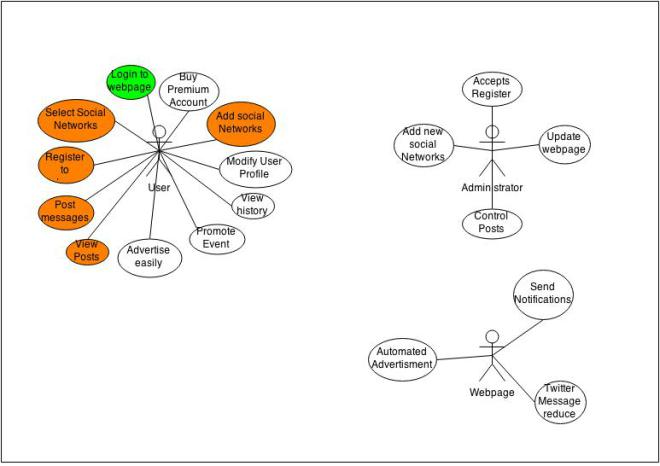
\includegraphics[width=16cm]{./img/usecase_socialfunnel.jpg}
\end{center}
	
To be determined
 
\subsection{Assumptions and Dependencies}

-Vorraussetzungen: Für den gebrauch der Anwendung braucht der Nutzer einen Internetzugang, sowie einen Account bei einem der Sozialen Netzwerke, die eingebunden werden.
Auch muss er sich innerhalb der Webanwendung einmal in den gewünschten sozialen Netzwerken anmelden, um diese über den Account der Web-Anwendung nutzen zu können.

- Abhängigkeiten: Die Anwendung funktioniert nur, wenn die Zielsysteme (Sozialen Netzwerke) funktionieren. 
Sollte es auf einer der anderen Seiten Probleme geben, kann diese nicht angesprochen werden.


[This section describes any key technical feasibility, subsystem or component availability, or other project related assumptions on which the viability of the software described by this Software Requirements Specification may be based.]

\section{Specific Requirements}

To be determined

[This section of the Software Requirements Specification should contain all the software requirements to a level of detail sufficient to enable designers to design a system to satisfy those requirements and testers to test that the system satisfies those requirements.   When using use-case modeling, these requirements are captured in the use cases and the applicable supplementary specifications.  If use-case modeling is not used, the outline for supplementary specifications may be inserted directly into this section.]


\subsection{Use-Case Reports}

To be determined

[In use-case modeling, the use cases often define the majority of the functional requirements of the system, along with some non-functional requirements.  For each use case in the above use-case model, or subset thereof, refer to, or enclose, the use-case report in this section.  Make sure that each requirement is clearly labeled.]

\subsection{Supplementary Requirements}

To be determined

[Supplementary Specifications capture requirements that are not included in the use cases.  The specific requirements from the Supplementary Specifications, which are applicable to this subsystem or feature, should be included here and refined to the necessary level of detail to describe this subsystem or feature.  These may be captured directly in this document or referred to as separate Supplementary Specifications, which may be used as an enclosure at this point. Make sure that each requirement is clearly labeled.]

\section{Supporting Information}

To be determined

[The supporting information makes the Software Requirements Specification easier to use.  It includes:

•           Table of Contents

•         Index

•         Appendices

 These may include use-case storyboards or user-interface prototypes. When appendices are included, the Software Requirements Specification should explicitly state whether or not the appendices are to be considered part of the requirements.]



\end{document}

